
%(BEGIN_QUESTION)
% Copyright 2008, Tony R. Kuphaldt, released under the Creative Commons Attribution License (v 1.0)
% This means you may do almost anything with this work of mine, so long as you give me proper credit

AC electric generators (sometimes called {\it alternators}) work on the principle of electromagnetic induction, spinning a magnet between wire coils as such:

$$\includegraphics[width=15.5cm]{i03256x01.eps}$$

These wire coils typically exist in pairs opposite each other from the centerline of the rotor shaft.  The wire coils are called {\it stator coils} or {\it stator windings}, because they are stationary.  This particular machine is called a {\it single-phase} alternator because the stator coils act as a single unit, producing one sine-wave AC voltage as the magnetized rotor turns.

\vskip 10pt

A {\it three-phase} AC generator has three sets of stator coils arranged 120$^{o}$ apart from each other around the centerline of the rotor shaft:

$$\includegraphics[width=15.5cm]{i03256x02.eps}$$

Since the three pairs of stator windings ``see'' the poles of the magnetized rotor pass by at different times, their respective sine-wave voltages will be out of step (out of phase) with each other.

\filbreak

The following graph shows the pattern of the AC voltage produced by the first alternator (single-phase), with only one stator coil pair, as the rotor makes two complete rotations (from 0$^{o}$ to 360$^{o}$, twice):

$$\includegraphics[width=15.5cm]{i03256x03.eps}$$

Sketch the patterns of the two additional AC voltages produced by the three-phase alternator on this same graph, and comment on the phase relationship between the three AC voltage waveforms.

\underbar{file i03256}
%(END_QUESTION)





%(BEGIN_ANSWER)

The three waves are phase-shifted 120$^{o}$ apart from each other, just as the three stator windings are arranged 120$^{o}$ apart from each other around the circle:

$$\includegraphics[width=15.5cm]{i03256x04.eps}$$
 
%(END_ANSWER)





%(BEGIN_NOTES)


%INDEX% Electronics review: 3-phase electrical power 

%(END_NOTES)


